\documentclass[titlepage]{scrartcl}
% Code Darstellung
\usepackage{listings}
\usepackage{listingsutf8}
\usepackage{multicol}

%lange Tabellen
\usepackage{longtable}
%Referenzen zwischen unterschiedlichen Dateien
\usepackage{xr}
\externaldocument{theorie}
\usepackage{lscape}
%Deutsche Sprachunterstützung
\usepackage[utf8]{inputenc}
\usepackage[ngerman]{babel}
\usepackage{marvosym}
\DeclareUnicodeCharacter{20AC}{\EUR}

%Für das Einbinden von Bildern
\usepackage{graphicx}

%Tabellen
\usepackage{array}

%Tabellen automatisch schoener
\usepackage{booktabs}

%Caption
\usepackage{caption}
\usepackage{subcaption}

%Formeln
\usepackage{mathtools}
\usepackage{amsmath}
\usepackage{amssymb}
\usepackage{amstext}
\usepackage{dsfont}

%\usepackage{mnsymbol}

% Interssante natbib Optionen: 
% numbers : Nummerierte Zitateinheiten
% sort&compress : Bei mehrfachen Zitaten, Sortierung und ggf. Verkürzungen
%\usepackage[]{natbib}

%Vectorpfeile schöner
\usepackage{esvect}

%Formatierung
\usepackage[T1]{fontenc}
\usepackage{lmodern}
\usepackage{microtype}

%Schaltbilder malen
%\usepackage[europeanresistors,cuteinductors,siunitx]{circuitikz}
\usepackage{comment}
\usepackage{csquotes}

%Formatierungsanweisungen
\newcommand{\wichtig}[1]{\underline{\large{#1}}}
\newcommand{\aref}[1]{Abb. \ref{#1}}
\newcommand{\R}{\mathbb{R}}
\newcommand{\K}{\mathbb{K}}
\newcommand{\C}{\mathbb{C}}

%Klickbare Referenzen
\usepackage[hidelinks]{hyperref}

\begin{document}

\section{Vorübung 1}

\begin{itemize}
\item Wahre Sonnenzeit (WZ): Die wahre Sonnenzeit wird am Stand der Sonne am Himmel gemessen und beträgt 12 Uhr, wenn die Sonne durch den Meridian des Standortes geht.
\item Mittlere Sonnenzeit (MZ): Die mittlere Sonnenzeit ist eine gleichmäßig vergehende Zeit, wobei eine fiktive mittlere Sonne den Zeitverlauf bestimmt.
\item Weltzeit, Universal Time (UT): Die Weltzeit ist ein Zeitmaß, das aufgrund internationaler Vereinbarungen für jeden Ort die gleiche Zeit liefert. Sie entspricht dabei der mittleren Sonnenzeit auf dem 0-Meridian.
\item Zonenzeit: Als Zonenzeit wird eine einheitliche Zeit innerhalb einer Zeitzone bezeichnet. Dabei wird die Erde in 24 Zeitzonen eingeteilt, um innerhalb einer Zeitzone vertretbare Abweichungen von der mittleren Sonnenzeit zu gewährleisten.
\item Julianisches Datum (JD): Das Julianische Datum gibt die Tage an, die seit dem 1. Januar -4712, 12 Uhr vergangen sind.
\item Sternzeit, Sidereal Time (ST): Die Sternzeit ist ein Zeitmaß, das auf der scheinbaren Rotation der Sterne am Himmel, hervorgerufen durch die Erdrotation, beruht. Ein Sterntag ist die Dauer, die der Sternenhimmel für ein ganze scheinbare Umdrehung benötigt.
\item Ephemeridenzeit (ET,TT oder TDT): Die Ephemeridenzeit ist ein durch die Dynamik des Sonnensystems definiertes Zeitmaß. Eine Ephemeridensekunde entspricht dabei dem 31.556.925,9747ten Teil eines Tropischen Jahres. 
\item Atomzeit: Die Atomzeit ist ein Zeitmaß das auf der SI-Sekunde basiert und wird weltweit bei zahlreichen Zeitinstituten in der Regel durch Cäsium-Atomuhren realisiert. Eine Sekunde ist das 9.192.631.770-fache der Periodendauer der dem Übergang zwischen den beiden Hyperfeinstrukturniveaus des Grundzustandes von Atomen des Nuklids Cs-133 entsprechenden Strahlung.
\end{itemize}

\section{Vorübung 2}

Streng gleichförmig verlaufen die mittlere Sonnenzeit, die Weltzeit, die Zonenzeit, die Ephemeridenzeit und die Atomzeit.

Die wahre Sonnenzeit verläuft aus zwei Gründen ungleichmäßig: Zum einen wird der gleichmäßige Verlauf durch die elliptische Form der Erdbahn und zum anderen durch die Neigung der Erdachse gestört.

Die Sternzeit steht unter dem Einfluss von Schwankungen der Rotation der Erde, wie z.B. die Präzession. Daher verläuft die Sternzeit nicht streng gleichförmig.

\section{Vorübung 3}

Der Verlauf der Zeitgleichung $ ZG=WZ-MZ $ ergibt sich hauptsächlich aus den beiden Ursachen:

\begin{itemize}
\item Elliptizität der Erdbahn
\item Neigung der Erdachse
\end{itemize}
Die Elliptizität der Erdbahn verursacht, dass sich die Erde in der Nähe des Perihels schneller bewegt als am Aphel. Daraus folgt ein Anteil der Zeitgleichung mit einer Periodizität von einem Jahr.

Die Neigung der Erdachse verursacht dagegen einen Anteil der Zeitgleichung mit einer Periodizität eines halben Jahres. Dieser Anteil entsteht dadurch, dass durch die Neigung der Erdachse, die effektive Drehgeschwindigkeit schneller ist, wenn von der Sonne aus gesehen die Projektion der Drehachse der Erde senkrecht auf der Ekliptik steht. (vgl. Abb. \ref{fig:Zeitgleichung})

\begin{figure}
        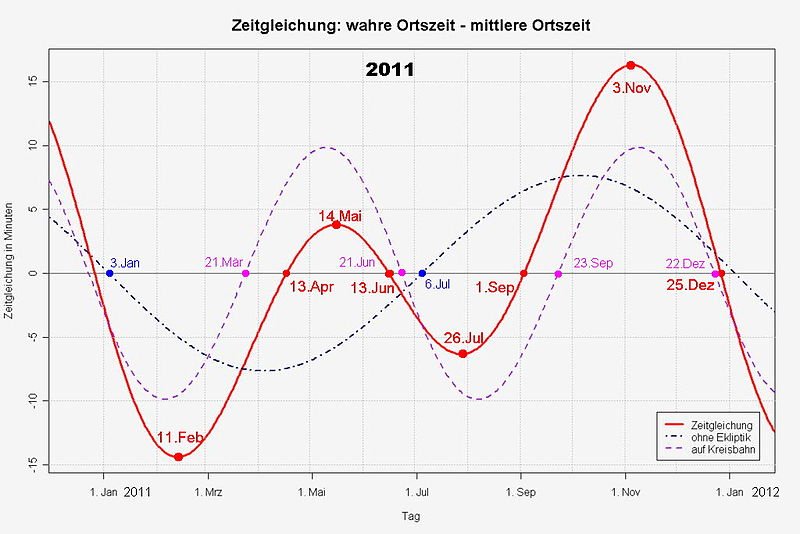
\includegraphics[width=.9\textwidth]{images/Zeitgleichung}
\caption{ Zeitgleichung in Minuten }
\label{fig:Zeitgleichung}
\end{figure}

\newpage

\section{Vorübung 4}
\subsection{Horizontsystem}

\begin{itemize}
\item Ursprung: Beobachter
\item Grundkreis: Horizont
\item Längen- und Breitenkoordinaten: Höhenwinkel und Azimut
\item Pole: Zenit und Nadir
\item Üblicher Verwendungszweck: Messungen auf der Erdoberfläche
\end{itemize}

\subsection{Festes Äquatorsystem}

\begin{itemize}
\item Ursprung: Beobachter oder Erdmittelpunkt
\item Grundkreis: Himmels-Äquator
\item Längen- und Breitenkoordinaten: Deklinationswinkel und Stundenwinkel
\item Pole: Himmelspole
\item Üblicher Verwendungszweck: Astronomische Beobachtungen
\end{itemize}

\subsection{Bewegliches Äquatorsystem}

\begin{itemize}
\item Ursprung: Erdmittelpunkt
\item Grundkreis: Himmels-Äquator
\item Längen- und Breitenkoordinaten: Deklinationswinkel und Rektazension
\item Pole: Himmelspole
\item Üblicher Verwendungszweck: Astronomische Beobachtungen
\end{itemize}

\subsection{Ekliptikales System}

\begin{itemize}
\item Ursprung: Sonnenmittelpunkt
\item Grundkreis: Ekliptik
\item Längen- und Breitenkoordinaten: ekliptikale Breite und Länge
\item Pole: Ekliptik-Pole
\item Üblicher Verwendungszweck: z.B. Berechnungen von Flugbahnen im Sonnensystem
\end{itemize}

\subsection{Galaktisches System}

\begin{itemize}
\item Ursprung: Sonnenmittelpunkt
\item Grundkreis: galaktische Ebene
\item Längen- und Breitenkoordinaten: galaktische Breite und Länge
\item Pole: galaktische Pole
\item Üblicher Verwendungszweck: z.B. Bestimmung der Rotationsgeschwindigkeit der Milchstraße
\end{itemize}

\begin{figure}
        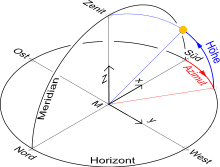
\includegraphics[width=.9\textwidth]{images/Horizontsystem}
\caption{ Horizontsystem }
\label{fig:Horizontsystem}
\end{figure}

\begin{figure}
        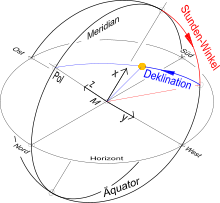
\includegraphics[width=.9\textwidth]{images/FestesAequatorsystem}
\caption{ Festes Äquatorsystem }
\label{fig:Festes Äquatorsystem}
\end{figure}

\begin{figure}
        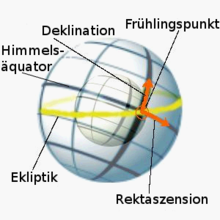
\includegraphics[width=.9\textwidth]{images/BewegtesAequatorsystem}
\caption{ Bewegliches Äquatorsystem }
\label{fig:Bewegtes Äquatorsystem}
\end{figure}

\newpage

\section{Vorübung 5}

Im Horizontsystem und im festen Äquatorsystem entsteht die zeitliche Variabilität eines Fixsterns durch die Erdrotation und durch die Parallaxe beim Umlauf der Erde um die Sonne. Der erstgenannte Effekt hat eine Periodizität von einem Tag, während die Periodizität des zweiten Effektes ein Jahr beträgt.

Dagegen entsteht die zeitliche Variabilität eines Fixsterns im beweglichen Äquatorsystem nur durch die Parallaxe bei Umlauf der Erde um die Sonne. Die Periodizität dieses Effekts beträgt natürlich auch ein Jahr.

\section{Vorübung 6}

Das Nautische Dreieck ist ein Hilfsmittel, um aus der Rektazension und der Deklination eines Sterns, seinen Azimut und seinen Höhenwinkel zu bestimmen. (vgl. Abb. \ref{fig:Nautisches Dreieck})

\begin{figure}
        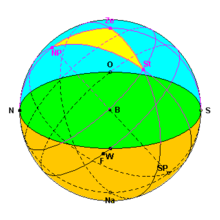
\includegraphics[width=.9\textwidth]{images/NautischesDreieck}
\caption{ Nautisches Dreieck }
\label{fig:Nautisches Dreieck}
\end{figure}

\end{document}